%------------------ vorlage.tex ------------------------------------------------
%
%
%-------------------------------------------------------------------------------


%------------------ Präambel ---------------------------------------------------
\documentclass[envcountsame, envcountchap, deutsch]{i-studis}
\usepackage{parskip} 
\usepackage[utf8]{inputenc}
\usepackage{glossaries}

\usepackage[a4paper]{geometry}
\usepackage[english, ngerman]{babel}
\usepackage{float}
\usepackage{nameref}

\usepackage[pdftex]{graphicx}
\usepackage{epstopdf}
\usepackage{subcaption}

\usepackage{listings}
\usepackage{makecell}

\usepackage[german, ruled, vlined]{algorithm2e}
\usepackage{amssymb, amsfonts, amstext, amsmath}
\usepackage{array}
%\usepackage[skip=10pt]{caption}
\usepackage[usenames, dvipsnames]{color}
\usepackage{xcolor}
%\usepackage{sectsty}
\usepackage{textcomp}
\usepackage{booktabs}
\usepackage{wrapfig}
\usepackage{titlesec}
\usepackage{blindtext}
\usepackage[shortcuts]{extdash}
% \usepackage{enumerate}
\usepackage{enumitem}
\usepackage{svg}

% Zitierpakete
\usepackage[style=apa,backend=biber, maxcitenames=2]{biblatex}
% \DeclareLanguageMapping{german}{english}
\usepackage[pdftex, plainpages=false, breaklinks=true]{hyperref}
\usepackage[babel, german=quotes]{csquotes}
\addbibresource{Literatur.bib}

\usepackage{makeidx}
\usepackage{multicol}
\setlength{\tabcolsep}{0.5em}                  % for horizontal padding in tables

% Einstellungen für Code-Listings
\lstset{
        basicstyle=\ttfamily\scriptsize,       % print whole listing small and in monospace
        keywordstyle=\color{blue}\bfseries,    % underlined bold black keywords
        identifierstyle=,                      % nothing happens
        commentstyle=\color{red},              % white comments
        stringstyle=\ttfamily,                 % typewriter type for strings
        showstringspaces=false,                % no special string spaces
        framexleftmargin=7mm, 
        tabsize=3,
        showtabs=false,
        frame=single, 
        rulesepcolor=\color{blue},
        numbers=left,
        linewidth=146mm,
        xleftmargin=8mm,
        captionpos=b
}

\graphicspath{ {./Abbildungen/} }

\hypersetup{
    colorlinks,
    linkcolor={black},
    citecolor={blue!50!black},
    urlcolor={blue!80!black}
}

\makeindex

\pagestyle{myheadings}
\setlength{\textheight}{1.1\textheight}

\makenoidxglossaries{}

\newglossaryentry{0 --- 5KillRounds}{
    name={0 --- 5 Kill Rounds},
    description={Wie viele Runden ein Spieler hat, in denen er entweder 0, 1, 2, 3, 4 oder 5 Kills macht}
}

\newglossaryentry{API}{
    name={API},
    description={Application Programming Interface: Eine Schnittstelle über die mit einer Programmiersprache Daten abgefragt werden können}
}

\newglossaryentry{CSV-Datei}{
    name={CSV-Datei},
    description={Comma-separated values}
}

\newglossaryentry{Deaths}{
    name={Deaths},
    description={Wie oft der Spieler gestorben ist}
}

\newglossaryentry{FirstKillInWonRounds}{
    name={First kill in won rounds},
    description={Wie oft das Team die Runde gewinnt, nachdem der einzelne Spieler das Opening gemacht hat}
}

\newglossaryentry{GrenadeKills}{
    name={Grenade kills},
    description={Wie viele Kills der Spieler mit einer Granate gemacht hat}
}

\newglossaryentry{KillDeathDifference}{
    name={Kill Death difference},
    description={Die Differenz zwischen Kills und Deaths (KDd = Kills $-$ Deaths)}
}

\newglossaryentry{KillperDeath}{
    name={Kill per Death},
    description={Die Relation zwischen der Anzahl der Tode und den gemachten Kills (Kills/Deaths)}
}

\newglossaryentry{KillperRound}{
    name={Kill per Round},
    description={Wie viele Kills ein Spieler durchschnittlich in einer Runde macht (Kills/Played Rounds)}
}

\newglossaryentry{Kills}{
    name={Kills},
    description={Wie oft der Spieler einen gegnerischen Spieler getötet hat}
}

\newglossaryentry{Name}{
    name={Name},
    description={Der Name des Spielers}
}

\newglossaryentry{OpeningKillRating}{
    name={Opening kill rating},
    description={Wie oft der Spieler ein Opening probiert hat und erfolgreich oder nicht erfolgreich war}
}

\newglossaryentry{OpeningKillRatio}{
    name={Opening kill ratio},
    description={Die Relation zwischen Opening Kills und Opening Deaths (Opening Kills / Opening Deaths)}
}

\newglossaryentry{OtherKills}{
    name={Other kills},
    description={Wie viele Kills der Spieler mit anderen Objekten, die nicht direkt eine Waffe sind, gemacht hat}
}

\newglossaryentry{PistolKills}{
    name={Pistol kills},
    description={Wie viele Kills der Spieler mit einer Waffe in der Kategorie `Pistol' gemacht hat}
}

\newglossaryentry{RifleKills}{
    name={Rifle kills},
    description={Wie viele Kills der Spieler mit einer Waffe in der Kategorie `Rifle' gemacht hat}
}

\newglossaryentry{Role}{
    name={Role},
    description={Welche Rolle ein Spieler in seinem Team einnimmt}
}

\newglossaryentry{RoundsWithKills}{
    name={Rounds with Kills},
    description={Die Anzahl in wie vielen Runden der Spieler einen Kill getätigt hat}
}

\newglossaryentry{SMGKills}{
    name={SMG kills},
    description={Wie viele Kills der Spieler mit einer Waffe in der Kategorie `SMG' gemacht hat}
}

\newglossaryentry{SniperKills}{
    name={Sniper kills},
    description={Wie viele Kills der Spieler mit einer Waffe in der Kategorie `Sniper' gemacht hat}
}

\newglossaryentry{SnipertoRifleratio}{
    name={Sniper to Rifle ratio},
    description={Das Verhältnis aus Sniper Kills zu Rifle Kills}
}

\newglossaryentry{Team}{
    name={Team},
    description={Zu welchem Team der Spieler Stand 18. Okt 2023 angehört}
}

\newglossaryentry{TeamWinPercentAfterFirstKill}{
    name={Team win percent after first kill},
    description={Wie oft das Team eine Runde gewinnt, wenn ein beliebiger Spieler ein Opening gemacht hat}
}

\newglossaryentry{TotalOpeningDeaths}{
    name={Total Opening Deaths},
    description={Wie oft der Spieler als erster in einer Runde gestorben ist}
}

\newglossaryentry{TotalOpeningKills}{
    name={Total Opening Kills},
    description={Die Anzahl an Runden, in denen der Spieler ein Opening gemacht hat}
}



%------------------ Titelseite -------------------------------------------------
\begin{document}
\setcounter{tocdepth}{4}
\setcounter{secnumdepth}{4}
\title{Anwenden des Knn-Algorithmus zur Vorhersage der Rollen in einem CS:GO Team}
\project{Seminararbeit}
% \degree{Bachelor of Science (B.Sc.)}                    % Nur bei Abschlussarbeit!
\address{im Studiengang Wirtschaftsinformatik an der\\Hochschule Trier}

\author{Niklas Metzen}
\supervisorFirst{Prof.\ Dr.\ Martin Vogt}
\matrikelnummer{977046}
\fachbereich{Wirtschaft}
\studiengang{Wirtschaftsinformatik}
\submitdate{\the\day.\the\month.\the\year}

\mytitlepage{}

%------------------ Vorwort, Kurzfassung, Verzeichnisse ------------------------
\frontmatter
\tableofcontents					% Inhaltsverzeichnis
\listoffigures                        % Abbildungsverzeichnis
\listoftables                           % Tabellenverzeichnis
%------------------ Kapitel ----------------------------------------------------
\mainmatter{}

%------------------ Kapitel 1 -------------------------------------------------------------

\chapter{Einleitung}
\section{Bedeutung von Daten und Veränderung des Multimediakontext}
Viel Zeit ist vergangen, seitdem der Archetyp eines `Gamers', als ein nur im Keller sitzenden, blassen und in seinen Fantasien verlorenen Teenager 
definiert war (\cite{Kowert_2014}). Heutzutage sind Videospiele in der Mehrheit akzeptiert und 
`Gamer' sind eine durch und durch diverse Gruppe an Menschen (\cite{Williams_2008}).
Durch die Diversifizierung des Publikums und das Platzieren in den Mainstream ist die Videospielindustrie im Jahr 2023 auf einen Umsatz von
406,2 Millionen US-Dollar gekommen (\cite{Clement_2023}). Das ist vergleichbar mit dem Umsatz der deutschen Automobilindustrie im Jahr 2021 (\cite{Klimaschutz_2023}). Es gibt 
für Unternehmen einen Anreiz diesen Wirtschaftsbereich zu bedienen, da für die Umsatzzahlen in den nächsten Jahren ein Aufwärtstrend 
prognostiziert wird (\cite{Clement_2023}). Einige Unternehmen spezialisieren sich auf den wettbewerbsorientierten teil der Video Spiel, den sogenannten E-Sport. 
Die größte Einnahmequelle von Kaptial für die Unternehmen, die professionelle Teams verpflichten, ist in der Form von Sponsoring (\cite{Tristão_2022}).
Unternehmen möchten die besten Sponsorships bekommen und Sponsoren sind daran interessiert,
die besten Organisationen zu sponsern, d.h die Organisationen welche im ihrem Bereich am erfolgreichsten sind. Das Ziel der Organisationen sollte
sein, die meisten Turniere oder Meisterschaften zu gewinnen, um die besten in ihrem Bereich zu werden. Um zu gewinnen, 
müssen die Organisationen die Spielweise der Gegner verstehen. 
Ähnlich wie im Schach gehöhren dazu Spielanalysen und diese Analyse benötigt Daten. Die Natur von wettbewerbsorientierten Videospiele ist es, dass diese aufgenommen, 
geteilt und archiviert werden können. 
Daten sind somit vorhanden und es können Analyseverfahren auf die Daten angewandt werden, um Erkenntnisse zu gewinnen.
Thema der Seminararbeit wird das Erklären und Anwenden von zwei beliebten Analysemethode anhand eines Fallbeispiels sein. 
\subsection{Fallbeispiel: Counterstrike: Global Offensive}

Counterstrike: Global Offensive (CS:GO) ist ein im Jahr 2012 veröffentlichter Online-Taktik-Shooter (\cite{Coropration_2012}).
Im Spiel geht es um zwei Teams die verschiedene Aufgaben erledigen müssen, um Punkte zu gewinnen. 
Die Teams werden in die sogenannten `Terroristen' und `Anti-Terroristen' aufgeteilt.
Die Terroristen müssen eine von zwei Aufgaben erledigen, um einen Punkt zu bekommem:

\begin{itemize}
    \item Das Terroristen Team beginnt die Runde mit einer Bombe, die ein Spieler im Inventar halten kann. 
    Die Terroristen müssen die Bombe auf einer von zwei 
    Bombenseiten (genannt A- und B-Site) legen und die Bombe vor den Anti-Terroristen verteidigen, bis diese nach einer gewissen Zeit explodiert.
    \item Alternativ können sie alle Mitglieder des Anti-Terroristen Teams töten, bevor die Rundenzeit abgelaufen ist.
\end{itemize}

Die Anti-Terroristen müssen eine der drei Aufgaben erledigen, um einen Punkt zu erlangen: 

\begin{itemize}
    \item Die Terroristen am Legen der Bombe auf einer Bombenseite hindern. Dies müssen sie solange machen bis die Rundenzeit abgelaufen ist.
    \item Alle Mitglieder des Terroristen Teams töten, bevor sie die Bombe gelegt haben.
    \item Nachdem die Terroristen die Bombe gelegt haben, die Bombe entschärfen bevor sie explodiert.
\end{itemize}

Nachdem ein Team eine der Aufgaben erledigt hat, gewinnt dieses Team die Runde und eine neue Runde beginnt. Die Runden haben ein Zeitlimit, läuft dieses aus, gewinnen automatisch die Anti-Terroristen. 
Das erste Team welches 16 Punkte erreicht, gewinnt das Spiel.
Der Spieler kann innerhalb einer Runde verschiedene Aktionen tätigen, um Geld zu verdienen. 
Dieses Geld kann für den Kauf von bestimmten Waffen und Utensilien benutzt werden, die es ermöglichen die eben genannten Aufgaben leichter zu erledigen. 
Neben dem Erledigen der Aufgaben müssen Teams auch auf ihre Wirtschaftlichkeit über die Runden hinaus achten.
Was CS:GO von anderen Taktischen Shootern unterscheidet ist, dass jeder Charakter im Spiel gleich ist.
Es gibt kein Levelsystem das reinen Zeitaufwand belohnt oder keine Waffe, die durch das Verwenden von echtem Geld stärker wird (\cite{TheWarOwl_2012}).
Wichtig allein, sind die individuellen Fähigkeiten die der Spieler, der den Charakter bedient, hat.
Eine tiefere Erklärung würde über den Rahmen dieser Seminararbeit hinaus gehen. Wie in anderen Sportarten haben sich
Ligen und Tuniere geformt. Der Spieleentwickler \textit{Valve Coropration}
hat im Jahr 2013 das erste professionell gesponsorte Tunier organisiert (\cite{Corporation_2013}).
Durch dieses Turnier konnten erstmalig CS:GO Spieler den Jobtitel `professioneller Videospieler' annehmen, sogenannte `Pro-Player'. 
Die vom Hersteller gesponsorten Tuniere, auch \textit{Major} gennant, gibt es ein bis zwei mal im Jahr (\cite{Mclaughlin_2023}) und werden als die wichtigsten
Turniere im gesamten Jahr angesehen. Zu den Tunieren werden die besten 24 Teams der Welt eingeladen (\cite{Magal_2023}).
Die Preisgelder die in diesen Turnieren ausgeschüttet werden sind erheblich. Das größte CS:GO-Turnier hatte einen Preispool von 2.000.000 US-Dollar (\cite{Strike_2021}).
Innerhalb der professionellen Welt hat es sich etabliert, dass, um das Erzielen der Aufgabe zu erleichten, die verschiedenen Teammitglieder
unterschiedliche Verantwortungen haben, während die Runde gespielt wird. Diese Verantwortung führt dazu, 
dass sich CS:GO von einem `Ballerspiel' zu einer Art Schach mit Waffen entwickelt in dem die Teams nicht nur mit Maus, Tastatur und Reaktionszeit 
gewinnen, sondern das taktische Denken ein integraler Bestandteil des Spiels wird. 
Das Team kann frei entscheiden, welche Rolle ein Spieler im Team erfüllen soll (\cite{TV_2023}).
In anderen Spielen ist die Rollenverteilung schon im Charakterdesign integriert, sodass eine Unterscheidung der Rollen der
Charaktere durch den Vergleich von Attributen einfach ist. Es gibt Spiele, die genau mit diesem Gedanken konzipiert sind (\cite{Entertainment_2019}). 
In CS:GO ist die Rollenaufteilung vom Spieler, nicht vom Charakter den er spielt, abhängig. Das Verhaltensmuster, das ein Spieler annimt, ist 
indikativ für die Rolle die der Spieler hat. Meine Frage ist, ob diese Verhaltensmuster/Rollen durch Daten, die während dem Spielen erhoben werden,
`sichtbar' gemacht werden können? Dieser Frage versuche ich in dieser Seminararbeit auf den Grund zu gehen.

\section{Ist es möglich, Rollen anhand von Daten vorherzusagen?}
Meine Frage ausformuliert ist, ob es möglich ist, mit einem aus dem Pro-Play gesammelten Datensatz, welcher die Rollen der Spieler beinhaltet, 
eine Voraussage machen zu können, welche Rollen ein Spieler hat, bei dem nur der Datensatz bekannt ist aber nicht die Rolle dieses Spielers?
Dieses Problem fällt, da es mehrerer Rollen gibt, in den Bereich der Klassifizierung, wobei die Rollen als Klassen betitelt werden. 
Ich werde mithilfe des K-Nächste-Nachbarn-Verfahren (Knn) ein prädiktives Modell aufstellen, welches diese Frage versucht zu beantworten.

%------------------ Kapitel 2 -------------------------------------------------------------

\chapter{Klassen wählen und aus Datenquelle diese extrahieren}
\section{Klassen = Rollen}
In CS:GO gibt es im Pro-Play bis zu 5 Rollen die in einem Team vertreten sind. Im Videospiel ist jeder Charakter gleich. Die Aktionen, die 
ein Spieler tätigt, zeigen welche Rolle die Person in dem Team hat. Folgende Rollen gibt es innerhalb eines Teams (\cite{TV_2023}):
\subsection{In-Game Leader (IGL)}
Der IGL kann wie ein Kapitän im Fußball verstanden werden. 
Der IGL ist ein Spieler, der die Taktiken und die Positionen auf der Karte, die alle Spieler im eigenen Team einnehmen sollen vorgibt. 
Runden beginnen mit einem festen Plan, den der IGL vorgibt. Je nachdem was das Ergebnis des Plans ist, muss der IGL aus dem Augenblick heraus 
eine neue Taktik überlegen, um die Runde zu gewinnen. Ein IGL muss vieles gleichzeitig bedenken.
\subsection{Entry Fragger (Entry)}
Der Entry ist der Spieler, welcher als erster auf eine Bombenseite läuft, mit dem Ziel, mindestens \textbf{Opening}\footnote{\textbf{Opening}: Der erste Kill innerhalb einer Runde.} zu erzielen.
Um somit dem Rest des eigenen Teams zu erlauben, auf die Bombenseite zu kommen, um die Bombe zu legen. Ein Entry muss eine schnelle 
Reaktionszeit haben und wissen, wo gegnerische Spieler auf der Bombenseite stehen könnten.
Ein Entry muss sehr aggressiv spielen und sich für den Erfolg des Teams opfern, selbst wenn er dabei nicht immer erfolgreich ist.
\subsection{Support}
Die Aufgabe eines Support ist in zwei Bereiche aufgeteilt:
\begin{enumerate}
    \item \textbf{Die Unterstützung des Entry}: Der Support ist nach dem Entry der zweite Spieler auf der Bombenseite und versucht entweder dem Entry 
    dabei zu helfen den gegnerischen Spieler zu töten oder wenn der Entry stirbt, einen \textbf{Refrag}\footnote{\textbf{Refrag}: Ein Gegner tötet ein Teammitglied und ein anderes Teammitglied tötet daraufhin den Gegner. Die Abfolge tritt häufig auf.} zu erzielen.
    \item \textbf{Lineups}: Der Support muss für alle Karten, auf allen Positionen wissen, welche Utensilien er verwenden kann, um das gegnerische 
    Team daran zu hindern, die Bombenseite zu verteidigen.
\end{enumerate}
\subsection{AWPer}
Die AWP ist ein Scharfschützengewehr, welches signifikant mehr in der Anschaffung kostet, es aber ermöglicht, mit nur einem Schuss, den gegnerischen 
Spieler zu töten. Die AWP ist jedoch langsamer in der Handhabung. Ein AWPer ist der Spieler im Team, der dediziert die AWP verwendet. 
Aufgabe ist es, Knotenpunkte auf der Karte zu halten und jeden gegnerischen Spieler der in das Zielfernrohr kommt, zu töten. 
Benötigt ist vom AWPer eine schnelle Reaktionszeit und das Wissen wie er sich richtig auf der Karte positionieren kann. 
\subsection{Lurker}
Der Lurker ist ein Spieler, der weit weg von seinem Team versucht Informationen über Positionen der Gegner zu bekommen oder die Karte so aufteilt, 
dass das gegnerische Team es nicht mehr schafft eine Bombenseite zu verteidigen. Wichtig ist die Bewegungen der gegnerischen Spieler 
voraussagen zu können, ein tiefes Verständnis darüber wie das gegnerische Team denkt und entscheiden zu können welche Informationen 
an den IGL weiterzugeben sind.
\section{Wählen einer Datenquelle}
\subsection{HLTV für Nachrichten und Statistiken zu CS:GO}
HLTV ist eine seit 2002 ins Leben gerufene News Webseite, die über die Geschehnisse im Pro-Play besonderes mit Augenmerk auf CS:GO berichtet (\cite{A/S_2015}). 
HLTV biete für Spiele von Tems einen Liveticker an. Die Daten, die mit dem Liveticker gesammelt werden, können später auf einem separaten 
Teil der Webseite nachgeschlagen werden.
\section{Verwendete Merkmale der Spieler}
Die auf dem separaten Teil der Webseite verfügbaren Statistiken, sind öffentlich zugänglich, da diese Daten direkt aus den Spiel entnommen werden. 
Die Vermutung liegt nahe, dass sie auch auch die Rolle eines Spielers innerhalb des Teams widerspiegeln können. Die Daten beziehen sich auf die letzen 12 Monate.

Folgende Merkmale\footnote{erklärt werden die Merkmale im Glossar} werden veröffentlicht:
\newline
\Gls{Name}, \Gls{Kills}, \Gls{Deaths}, \Gls{KillperDeath}, \Gls{KillperRound}, \Gls{RoundsWithKills}, \Gls{KillDeathDifference}, \Gls{TotalOpeningKills}, 
\Gls{TotalOpeningDeaths}, \Gls{OpeningKillRatio}, \Gls{OpeningKillRating}, \Gls{TeamWinPercentAfterFirstKill}, \Gls{FirstKillInWonRounds}, 
\Gls{0 --- 5KillRounds}, \Gls{RifleKills}, \Gls{SniperKills}, \Gls{SMGKills}, \Gls{PistolKills}, \Gls{GrenadeKills}, \Gls{OtherKills}, \Gls{Role}, \Gls{Team}
, \Gls{SnipertoRifleratio}

\section{Semi-Manuelle Extraktion von Daten aus HLTV}
HLTV bietet keine \Gls{API} an, die es ermöglicht die Daten über eine Programmierschnittstelle zu exportieren. Es ist jedoch möglich aus dem Browser die 
Statistiken der einzelnen Spieler herunterzuladen. Die heruntergeladene Datei ist im HTML-Format. Die Daten werden mittels einem \textbf{HTML-Scraper}\footnote{\textbf{HTML-Scraper}: Eine Technologie mit der gezielt Daten aus textähnlichen Dateien extrahiert werden können.} extrahiert. 
Die HTML-Dateien wurden in einem Ordner gespeichert, ich iteriere mit einem selbst geschriebenen Python Skript über 
die Dateien im Ordner und lese aus den gegebenen Tabellen die Daten aus. Die Daten werden dann geordnet in eine \Gls{CSV-Datei} geschrieben. In der \Gls{CSV-Datei}
sind dann 26 Merkmale. In der HTML-Datei ist jedoch nicht hinterlegt, welche Rolle der Spieler in seinem Team übernimmt. Aus einer Enzyklopädie kann 
jedoch entnommen werden, welche Rolle ein Spieler hat (\cite{Landsmann_2021}).
Ich erstelle eine \Gls{CSV-Datei} mit den Spielernamen und den Rollen im Team. Über ein Pandas Data Frame konsolidiere ich die Datensätze und exportiere 
diese als finale \Gls{CSV-Datei}.

%------------------ Kapitel 3 -------------------------------------------------------------

\chapter{Verwendete Methoden zur Rollenfindung}
\section{Principal Component Analysis (PCA) zum generieren neuer Merkmale}
Principal component analysis, zu Deutsch Hauptkomponentenanalyse, ist ein Verfahren der multivariaten Statistik, die hochdimensionale Datensätze mit neuen voneinander 
unabhängigen Komponenten, so gut wie möglich erklären soll. Die neuen Komponenten sind Linearkombinationen aus den originalen Merkmale.
Die Anzahl der neuen Komponenten ist gleich der Merkmale im vorherigen Datensatz und erklären die Daten so gut wie die ursprünglichen 
Merkmale es auch tun. Die neuen Komponenten zielen darauf ab, dass die ersten Komponenten die Daten so gut wie möglich beschreiben können. Die Restlichen Komponenten haben nur einen 
marginalen Beitrag zu der Erklärungsfähigkeit der Daten (\cite[p.2]{Lavrenko_Sutton_2011_pca}).

\subsection{Warum PCA verwenden?}
Die Güte von bestimmten Data Mining Algorithmen leidet unter dem `Curse of dimensionality'. Eine Dimension ist hierbei ein Merkmal, dass das beobachtete Objekt haben kann 
(z.B. Größe, Alter oder Beziehungsstatus). Hochdimensionale Daten haben sehr viele mögliche Kombinationen, in denen die Observationen vorkommen können. 
Die Zahl der möglichen Kombinationen steigt mit jeder neuen Dimension an. 
Bei steigender Dimensionsanzahl werden die potentiell möglichen Merkmalsausprägungen weniger durch die tatsächlichen Merkmalsausprägungen `ausgefüllt'. 
Bei Verfahren, jene die Distanz zwischen den Datenpunkten verwenden, um die Zugehörigkeit zu Klassen darzustellen, ist es bei weit auseinanderliegenden Datenpunkten schwierig, eine
Zugehörigkeit der Datenpunkte zur gleichen Klasse zu rechtfertigen, da die Datenpunkte zueinander über keine Homogenität verfügen.
Zwei Wege den `Curse of dimensionality' zu reduzieren sind: Die Stichprobengröße erhöhen, sodass sehr viele der 
möglichen Kombinationen abgedeckt werden, oder die Dimensionen der Daten müssen reduziert werden, damit die Gesamtmenge der möglichen Kombinationen sinkt (\cite{Altman_Krzywinski_2018}).
Die Größe der Stichprobe anzupassen ist nicht immer möglich. Dimensionsreduktion, ist nach der Erhebung einer Stichprobe, immer noch möglich und kann 
bei einer begrenzten Stichprobengröße das Rauschen der Daten verringern. Es gibt zwei Methoden die Dimensionen von Daten zu reduzieren:

\begin{itemize}
    \item \textbf{Feature selection}, dabei werden die zu verwendenden Merkmale vor dem Anwenden des Verfahrens gewählt. 
    Ob die Kombination von ausgewählten Merkmalen einer hohen Qualität entsprechen, kann erst nach der Anwendung der Analysemethode durch z.B. 
    Information Gain oder einem anderem Qualitätsmerkmal (basierend auf der Angewendeten Analysemethode) gemessen werden. Da dies jedoch eine Art `Trail and Error' bedingt, 
    ist es wünschenswert andere Arten von Dimensionsreduktion zu finden (\cite[p.2]{Lavrenko_Sutton_2011_pca}).
    \item \textbf{Feature extraction}, dabei werden basierend aus gewichteten Kombinationen von den vorhandenen Merkmalen neue, voneinander unabhängige Merkmale bestimmt. 
    Von diesen neuen Merkmalen können weniger Merkmale ausgewählt werden, die Daten jedoch zum größten Teil erklären (\cite[p.2]{Lavrenko_Sutton_2011_pca}).
\end{itemize}
\subsection{Grundlagen für PCA}
\subsubsection{Warum Varianz in Daten für Klassifikation wichtig ist}
Bei einer Klassifikation ist vorteilhaft, wenn die Datenpunkte und die dazugehörigen Klassen, untereinander homogen und voneinander heterogen in ihren Merkmalsausprägungen sind.
Wenn die Punkte nah aneinander sind, dann unterscheiden sich die Klassen auf dieser Gerade respektiv ihrer Merkmalsausprägungen nicht stark und 
die Gerade ist schlecht darin Unterschiede in den Klassen darzustellen (Abbildung~\ref{fig:var_max}). Dieses Verständnis kann auf den $n$-Dimensionalen Raum angewandt werden. 
Varianz lässt sich als ein Maß der Entfernung von Datenpunkten zu einem Mittelpunkt einer Merkmalsausprägung verwenden. Damit beschrieben werden kann welchen Beitrag zur Erklärungsfähigkeit eine Komponente bei der Klassifikation hat, 
ist hoher Varianz-Wert somit Erstrebenswert (\cite[p.3]{Lavrenko_Sutton_2011_pca}).

\vspace{1ex}
\begin{figure}
    
\includegraphics[width=\textwidth]{comparison_variance_two_points.drawio.png}
    \caption{Visuallisierung, das eine erhöhte Varianz in der Klassifikation von Vorteil ist}
\end{figure}

\subsection{Ablauf PCA}
Im Verfahren werden zuerst von allen Punkten der Mittelwert aller Merkmale berechnet und diese werden von allen Merkmalsausprägungen der Datenpunkte abgezogen.
Der neue Mittelwert beträgt $0$, dies erleichtet die Mathematik, auf der PCA beruht, verändert aber den relativen Abstand der Datenpunkte voneinander nicht.
PCA erstellt einen initialen Vektor, der alle Dimensionen des Datensatz beinhaltet, bei $n$-Dimension beinhaltet der Vektor $n$-Elemente. 
Zur Erklärung gehe ich von zwei Dimensionen aus, PCA kann auf den $n$-Dimensionalen Raum angewandt werden.
Daraufhin werden alle erhobenen Datenpunkte auf eine Gerade, die den Vektor als Richtung hat, projiziert. 
Sind die Datenpunkte auf die Gerade Projiziert, wird die Varianz der projizierten Punkte berechnet. 
Daraufhin wird auf den vorherigen Vektor orthogonal ein weiterer Vektor gespannt, dieser weitere Vektor spannt dann wieder eine Gerade, auf den die ursprünglichen 
Datenpunkte projiziert werden. Daraufhin wird wieder die Varianz der Gerade berechnet. Dies wird so lange gemacht, bis es nicht mehr möglich 
ist einen orthogonalen Vektor zu spannen. Um sicher zu gehen, dass der erste Vektor optimal ist, beziehungsweise, dass die Varianz der Gerade, die auf den Vektor gespannt wird, maximal ist,
kann wie in Abbildung~\ref{fig:var_max} die Richtung des Vektors (Somit auch die Steigung der Geraden) angepasst und die Varianz der projizierten Punkte neu bestimmt werden.
Dies wird solange gemacht bis die größte Varianz gefunden wurde.
\begin{figure}
    \centering

    \begin{subfigure}{0.45\textwidth}
        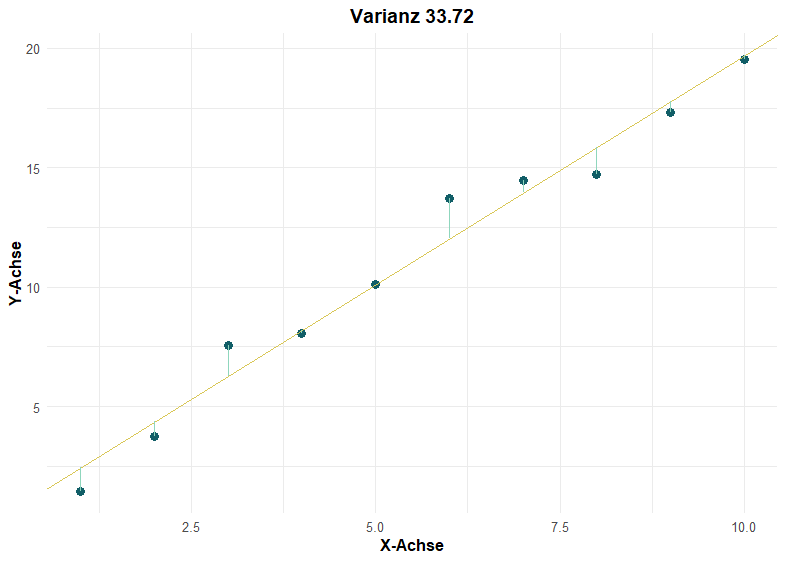
\includegraphics[width=\linewidth]{projected_points_to_line.png}
    \end{subfigure}
    \hfill
    \begin{subfigure}{0.45\textwidth}
        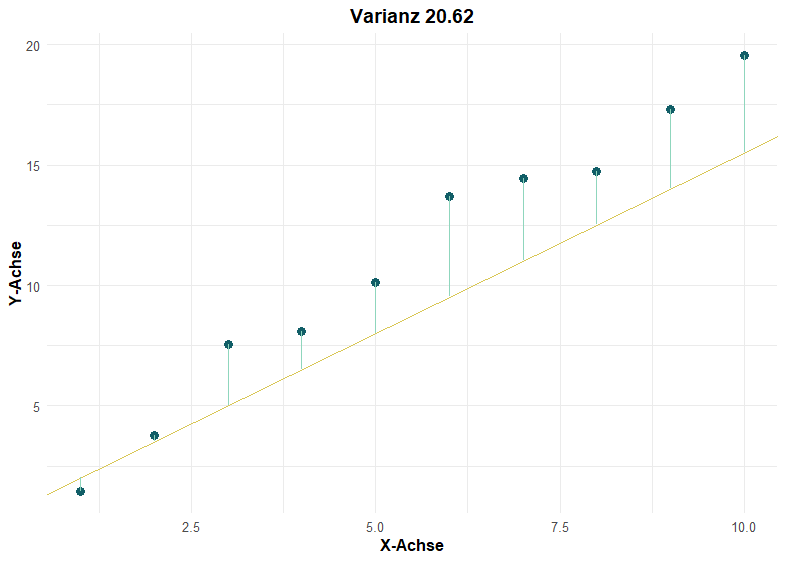
\includegraphics[width=\linewidth]{projected_points_to_line_low_variance.png}
    \end{subfigure}
    \caption{Veränderung der Varianz beim Rotieren des Vektors}\label{fig:var_max}
\end{figure}

Die Vektoren mit der größten Varianz sind diese, die die Daten am besten beschreiben. Die nach Varianz-Wert absteigend geordnete Übersicht der Vektoren sind die 
Hauptkomponenten. Der Vektor, der die größte Varianz hat, ist die erste Hauptkomponente, der mit der zweitgrößten, die zweite 
Hauptkomponente und so weiter. Die Anzahl der Hauptkomponenten ist gleich mit der Anzahl der Merkmale im Datensatz. In einem sogenannten 
Scree-Plot lassen sich die prozentualen Anteile, die die Hauptkomponenten die Daten erklären, darstellen.
Das Teilen der $i$-ten Varianz durch die Summe aller Varianzen ist der Anteilswert den der $i$-te Vektor an der Erklärung der Daten hat.
\begin{align}
    \textnormal{Anteil an der Erklärung des Vektors}_{i} = \frac{var_{i}}{\sum _{i=1}^{n} {var_{i}}} 
\end{align}

\subsection{Gewählte Merkmale}
Auf mein Beispiel angewendet und in einen Scree-Plot (\ref{fig:screeplot}) visualisiert, wähle ich die ersten sechs Hauptkomponenten und dessen Werte für die weitere Verwendung aus, diese sechs Hauptkomponenten erklären
$96,5\%$ der Daten.

\vspace{1ex}
\begin{figure}
    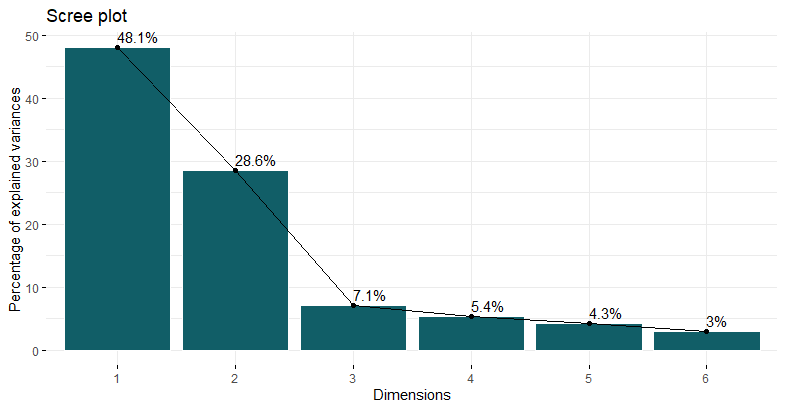
\includegraphics[width=\textwidth]{screeplot.png}
    \caption{Prozentualer Anteil der Erklärungsfähigkeit der einzelnen Hauptkomponenten vom gesamten Datensatz}\label{fig:screeplot}
\end{figure}

Das Reduzieren auf die ersten zwei Hauptkomponenten in Abbildung~\ref{fig:first_two_pc_plotted} ermöglicht auch eine Visuallisierung, die schon einen ersten Beweis geben kann, dass die Rollen (zumindestens für die Rolle `AWP') innerhalb CS:GO auch mit den erhobenen Daten 
bestimmt werden kann.

\vspace{1ex}
\begin{figure}
    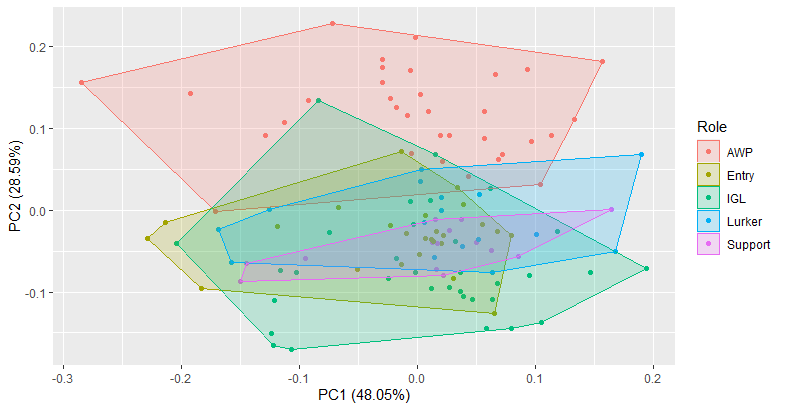
\includegraphics[width=\textwidth]{pc_plotted_roles_with_frame.png}
    \caption{Streudiagramm der zwei ersten Hauptkomponenten und deren projizierten Punkte. Die Einfärbung der Rollen ist basierend auf den Daten}\label{fig:first_two_pc_plotted}
\end{figure}

\section{K-nearest neighbors algorithm (Knn) zur Rollenfindung}
K nearest neighbors (Knn) ist ein Data Mining Klassifikationsalgorithmus, der auch auf Datensätze mit mehr als nur zwei Klassen angewendet werden kann.

\subsection{Funktionsweise von Knn}
\vspace{1ex}
\begin{figure}
    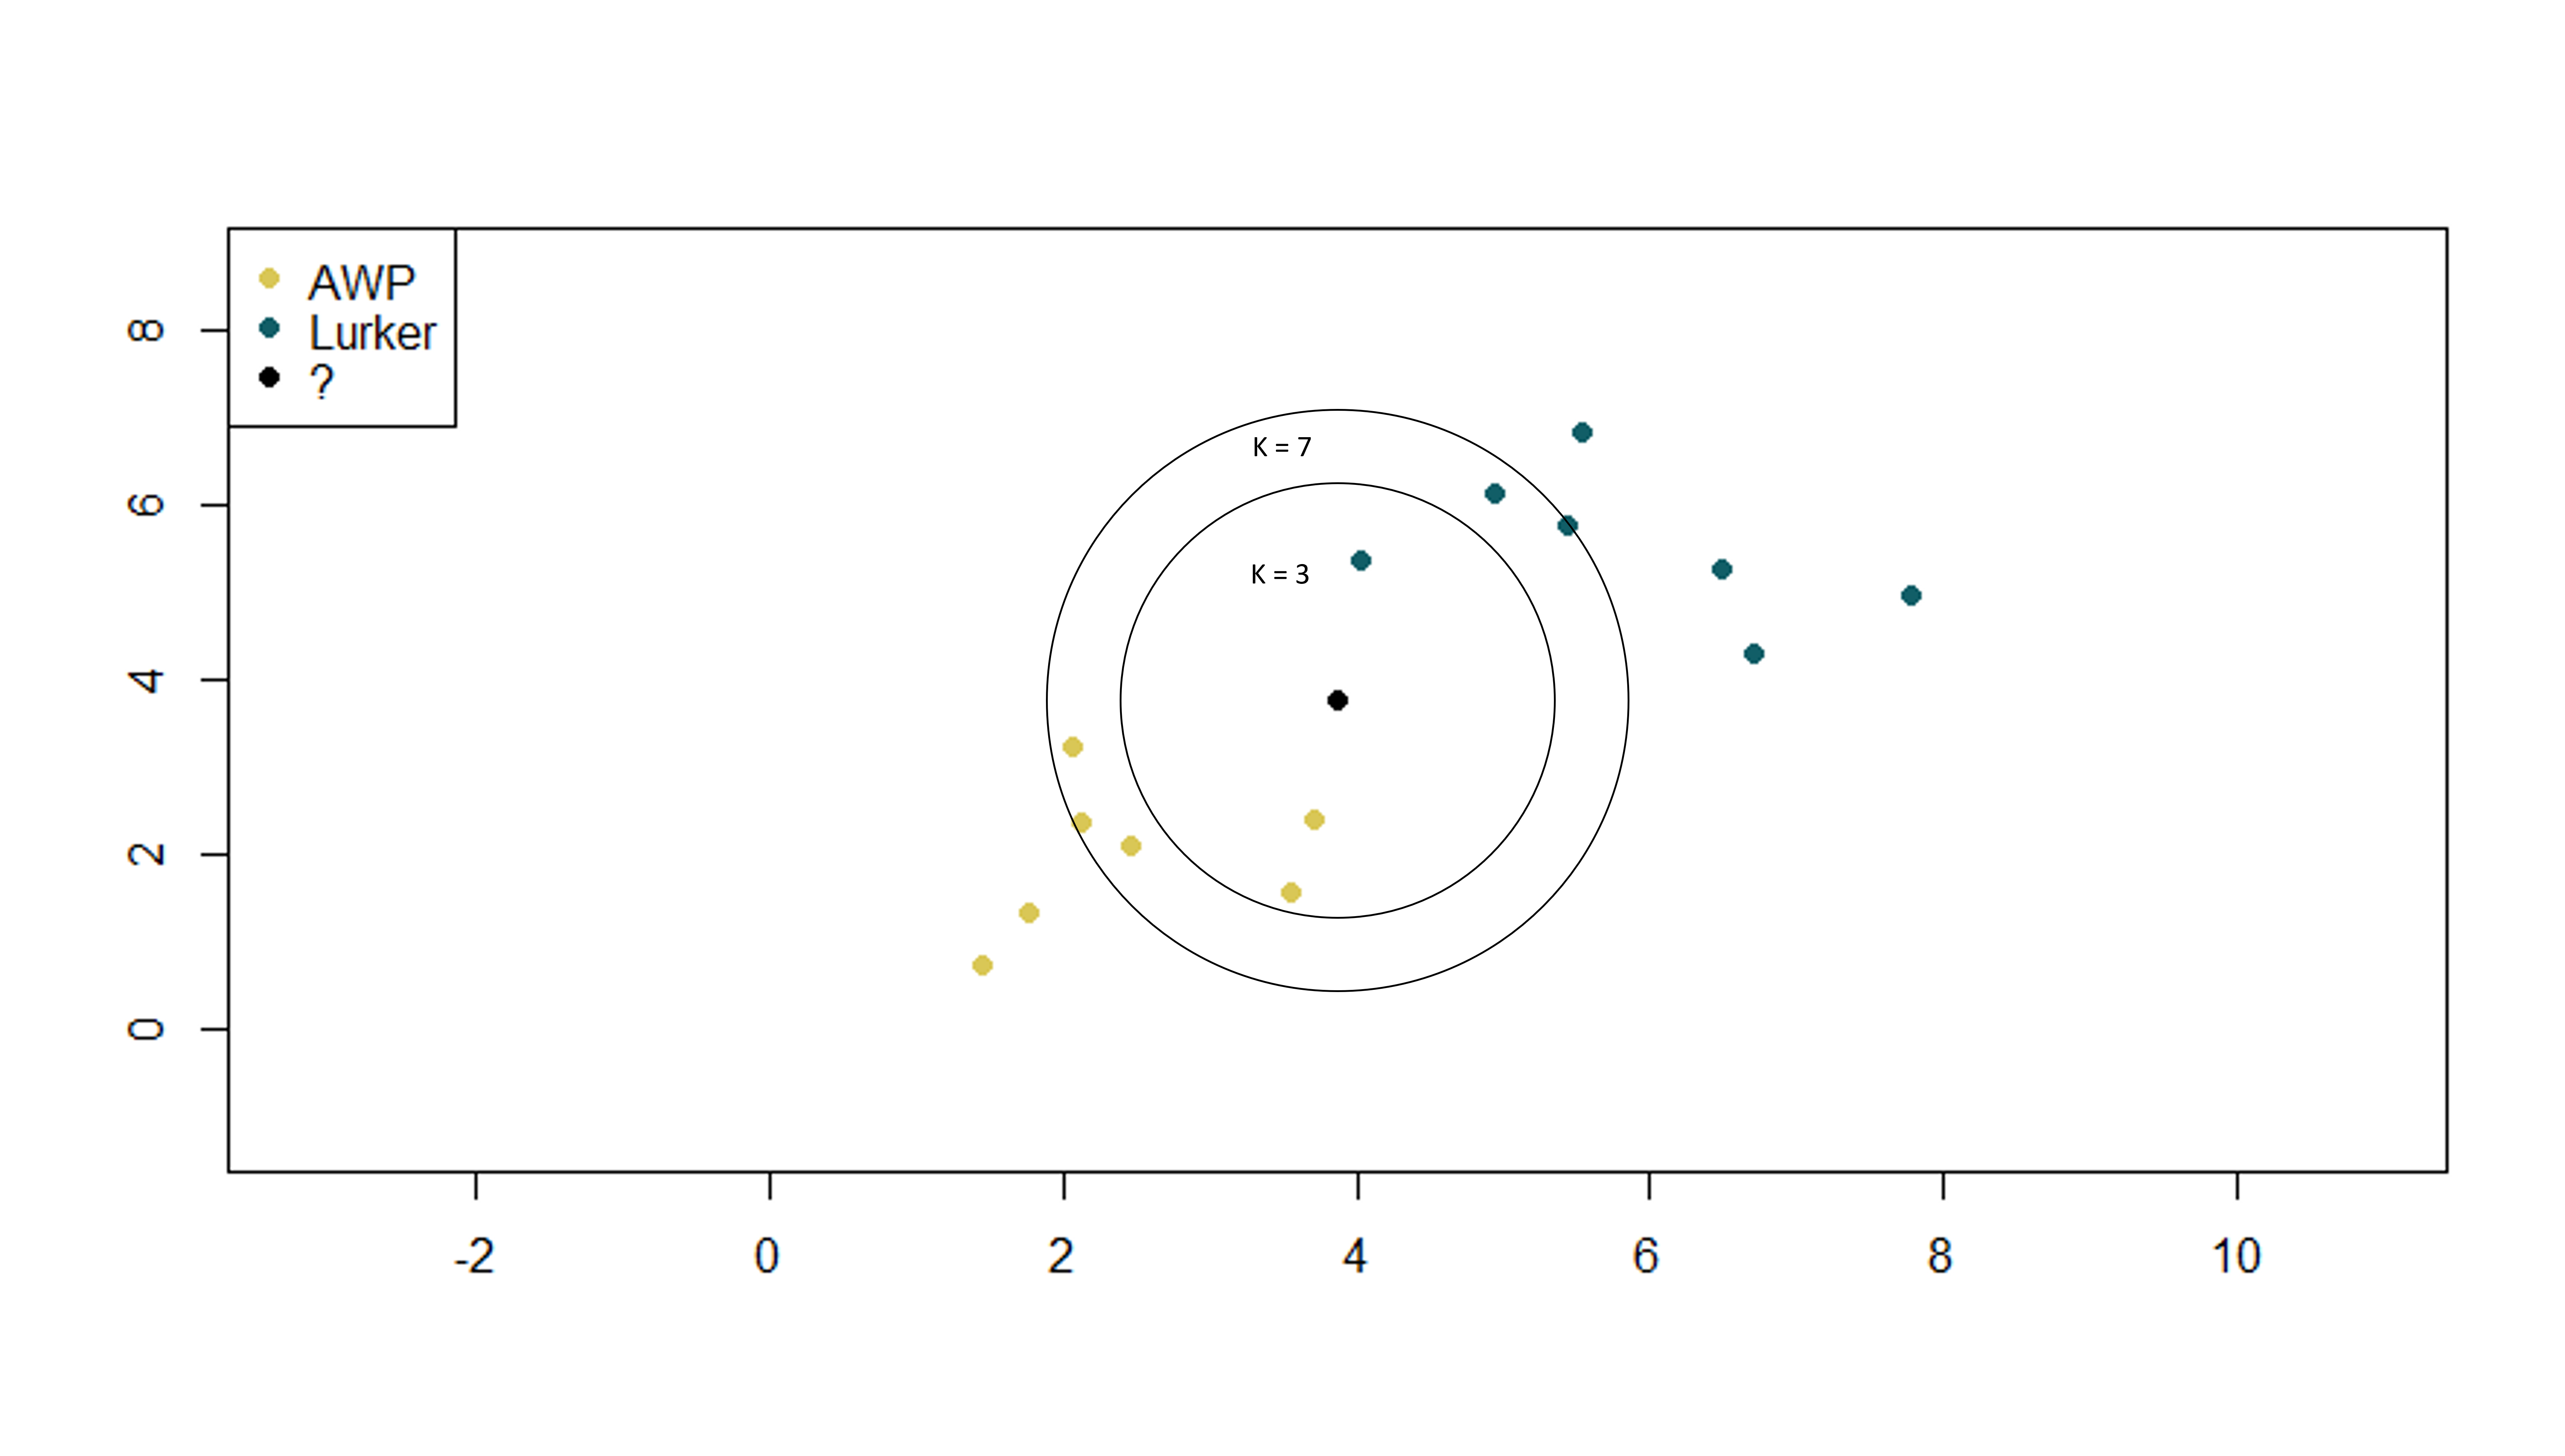
\includegraphics[width=\textwidth]{knn_circles.png}
    \caption{Die nächsten drei und sieben Datenpunkte um, einen Datenpunkt gezeichenet, bei denen die Klasse nicht bekannt ist.}\label{fig:knn_circles}
\end{figure}

\begin{table}
    \centering
    \begin{tabular}{lcccccl}
        \toprule 
        & \multicolumn{1}{c}{$k=3$} & \multicolumn{1}{c}{$k=7$}
        \\\cmidrule(lr){2-2}\cmidrule(lr){3-3}
        $Klasse$ & $Anzahl$ & $Anzahl$ \\
        $AWP$    &   $2$     & $5$       \\
        $Lurker$ &   $1$     & $3$       \\\bottomrule
    \end{tabular}
    \caption{Auflistung der Klassen der $k$ nächsten Nachbarn für den unklassifizierten Datenpunkt in Abbildung~\ref{fig:knn_circles}}\label{tab:majority_rule}
\end{table}
Knn vergleicht die neuen Datenpunkte, mit den k nächsten Datenpunkten, für die die Klassifikation schon bekannt ist (Abbildung~\ref{fig:knn_circles}).
K ist dabei eine selbst gewählte Anzahl an Datenpunkten. K ist maximal so groß, wie die Anzahl der Datenpunkte in der gewählten Stichprobe. 
Basierend auf den Klassen der nächsten Datenpunkte wird daraufhin eine Mehrheitswahl gemacht (Tabelle~\ref{tab:majority_rule}).
Die Klasse die am meisten vorkommt, ist die, die dem neuen Datenpunkt zugeteilt wird. 

In dem Beispiel aus Abbildung~\ref{fig:knn_circles} würde der neue Datenpunkt die Klasse: $AWP$ zugeordnet bekommen. Im Knn-Verfahren gibt es drei wichtige Komponenten:

\begin{itemize}
    \item Die Anzahl der verwendeten Merkmale für die Datenpunkte.
    \item Das Distanzmaß, welches den Abstand zwischen den Datenpunkten misst.
    \item Die für K gewählte Anzahl an zu vergleichenden Datenpunkten. 
\end{itemize}

\subsubsection{Die Euklidische Distanz als adäquates Distanzmaß}
Das Abstandsmaß ist eine Schlüsselkomponente, die die Güte der Analyse stark beeinflusst. Es gibt mehrere Abstandsmaße die verwendet werden können. 
Bei Daten mit metrischen Werten wird überwiegend die Euklidische Distanz verwendet.

\begin{align}
    d\left( p,q\right)   = \sqrt {\sum _{i=1}^{n}  {\left( q_{i}-p_{i}\right)}^2 }\label{eq:euklidische_distanz}
\end{align}

Wobei die Laufvariable $i$, für die Anzahl der Merkmale die erfasst wurden, steht $q$ für die Merkmalsausprägung des neuen Datenpunkt und $p$ für einen der Datenpunkte der schon eine Klasse hat. Bei Daten mit kategorischen Werten kann die Manhattan-Metrik verwendet werden. 
Weitere Abstandsmaße können verwendet werden. Wichtig ist es, ein Abstandsmaß zu wählen, dass alle Dimensionen gleichmäßig in dem resultierenden 
Abstandsmaß inkludiert. Das Problem der Euklidischen Distanz ist, dass sie sehr sensibel gegenüber Ausreißern ist.
\subsubsection{Die Bestimmung des richtigen K-Wertes}
Die Wahl des richtigen K ist wichtig, da die Abstimmung über die Klasse des unklassifizierten Datenpunktes lokal stattfindet und nicht direkt von der Gesamtmenge der Datenpunkte abhängig ist. Vorab zusagen ist, dass 
es keinen Algorithmus gibt, der die Anzahl von K richtig wählt. Wenn das K sehr klein ist z.B. $K = 1$, dann wird die nächste Klasse, die neben 
dem Datenpunkt liegt, als Voraussage verwendet.
Wenn nun aber Ausreißer oder Fehler in den Daten existieren, dann kann die Wahl des nächsten Nachbar dazu führen, 
dass Rauschen oder falsch gelabelte Daten, die Ergebnisses verfälscht (Abbildung~\ref{fig:knn_wrong_label}).  

\vspace{1ex}
\begin{figure}
    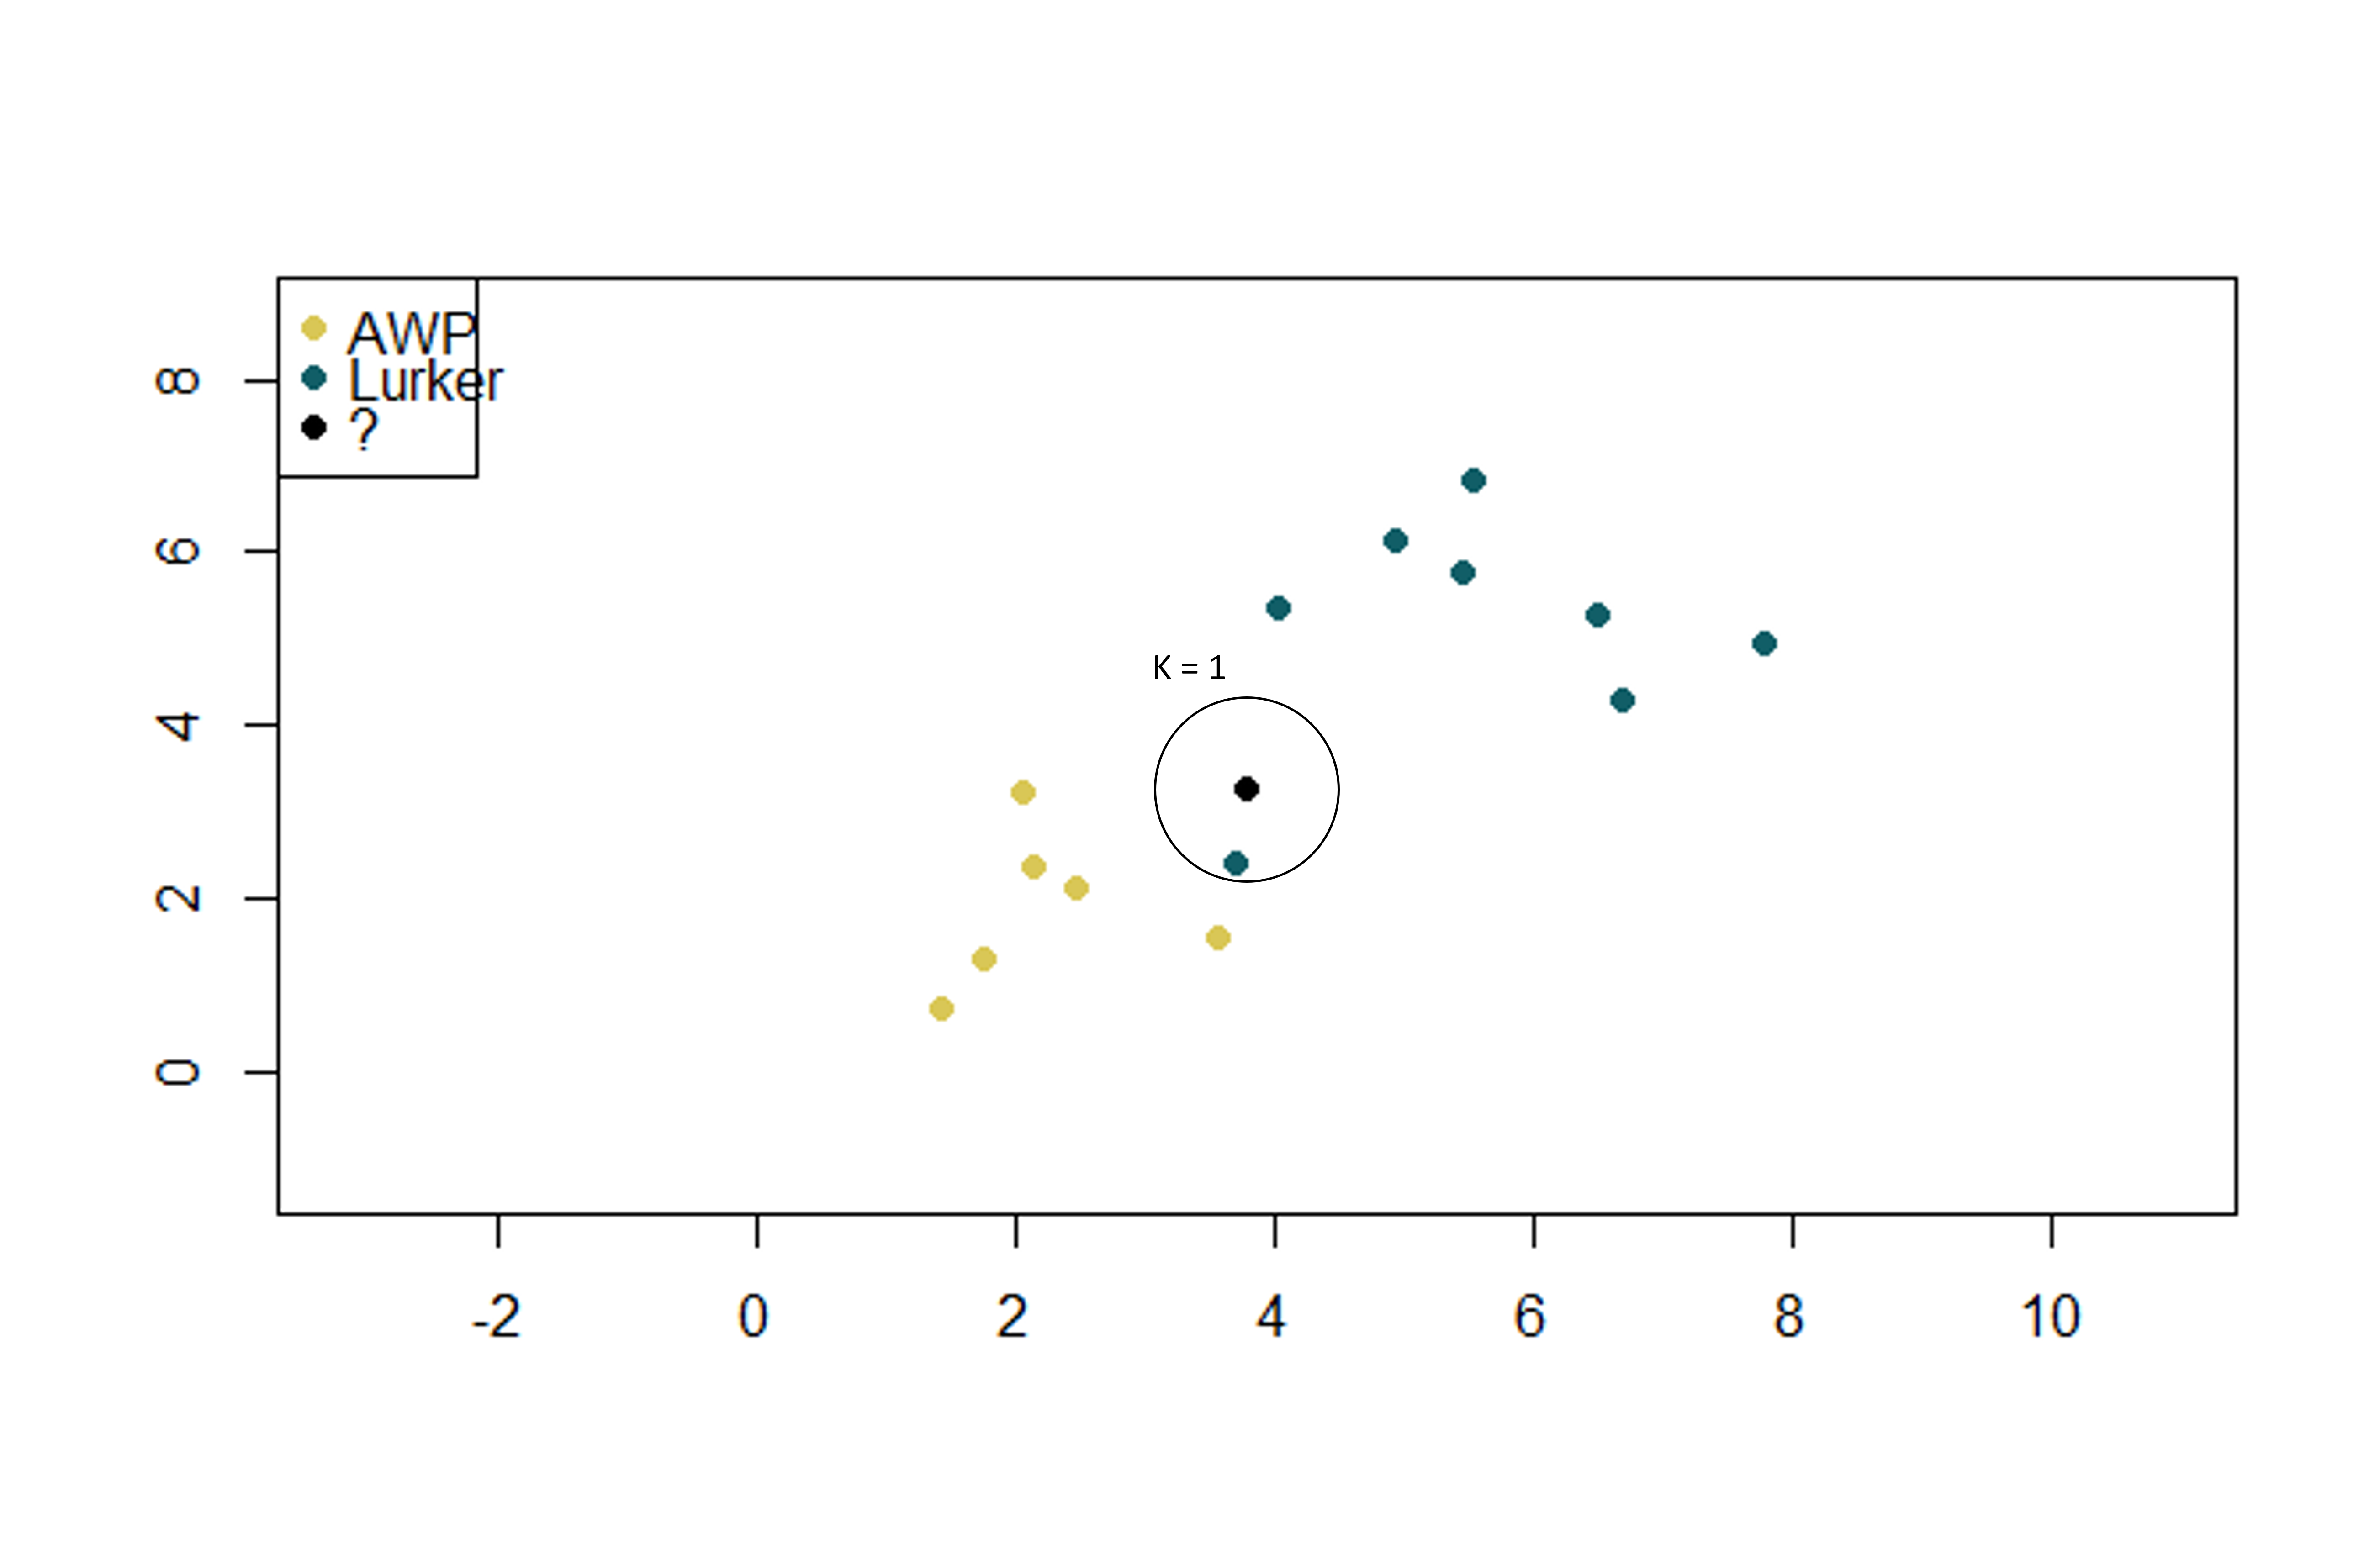
\includegraphics[width=\textwidth]{knn_wrong_label_circled.png}
    \caption{Falsche Klassifizierung durch z.B. falsch beschriftete Daten}\label{fig:knn_wrong_label}
\end{figure}

Wenn K nun sehr groß ist z.B. K = Anzahl der Datenpunkte, dann tendiert Knn dazu, die Klasse zu wählen, die am häufigsten in den Daten vorkommt (\cite{Lavrenko_Sutton_2011_knn}). 
Um den richtigen Wert für K zu finden, muss mit dem Datensatz iterativ eine Anzahl bestimmt werden. Die Daten werden in Trainings- und Testdaten 
aufgeteilt, um später die geschätzte Klasse mit der Tatsächlichen vergleichen zu können. Dabei ist es wichtig K nicht zu groß oder zu klein zu wählen. 
Der Knn-Algorithmus wird mit variierender Anzahl von K mehrmals angewendet. Über die Trefferquote habe ich dann die Güte des gewählten K bestimmt. 
Je höher die Trefferquote, desto besser das gewählte K.
\subsubsection{Probleme, die das Knn-Verfahren hat}
\begin{enumerate}
    \item Wenn es nur zwei Klassifizierung in den Daten gibt, kann es zu einem unentschieden bei der Wahl der Klassifikation kommen. Mit der Wahl eines ungeraden K-Wert (wie in Tabelle~\ref{tab:majority_rule}) wird dieses Problem behoben (\cite[p.4]{Lavrenko_Sutton_2011_knn}). Dies funktoniert jedoch nicht bei Daten mit mehr als zwei Klassen.
    \item Wenn ein Unentschieden in der Mehrheitswahl existiert, kann entweder zufällig einer der Klassen zugewiesen werden oder die im Datensatz am häufigsten vorkommende Klasse wird gewählt.
    \item Knn kann keine fehlenden Werte haben, fehlende Merkmalsausprägungen müs\-sen eine Zuweisung bekommen. Substituiert werden kann dann z.B. der Mittelwert der Merkmalsausprägung. Bei Daten mit kategorialen Merkmalen wird die am häufigsten vorkommende Ausprägung substituiert.
    \item Das größte Problem vom KNN-Verfahren ist der Rechenaufwand. Der Algorithmus muss immer alle Distanzen zu dem neuen Datenpunkt berechnen. Bei einer Menge von $n$-Datenpunkten und $d$-Merkmalen, entspricht der Rechenaufwand $O(nd)$.
\end{enumerate}

Um den Rechenaufwand zu minimieren gibt es Lösungen: 

\begin{itemize}
    \item Die Anzahl der erhobenen Merkmale kann durch das Auslassen von ausgewählten Merkmalen reduziert werden.
    \item Durch eine Hauptkomponentenanalyse kann die Anzahl der Merkmale gemindert werden.
    \item Die Verteilung der Datenpunkte werden z.B. durch die Aufteilung in einen K-D-Baum optimiert. Dieser Baum arbeitet mit Quantilen, um die Datenpunkte aufzuteilen und eine spätere Berechnung der Distanz auf weniger Datenpunkte zu beschränken (\cite{Lavrenko_Sutton_2011_knn}).
\end{itemize}

\subsection{Anwendung von Knn}
Die Güte von Knn leidet auch unter dem `Curse of dimensionality' deswegen sollte eine Auswahl der Merkmale vor der Anwendung bestimmt werden (\cite{6065061}).
Damit die Merkmale miteinander vergleichbar sind, normiere ich sie vor dem Anwenden des Verfahrens. Ich habe mit dem PCA-Verfahren die Hauptkomponenten bestimmt. Ich führe das Verfahren jeweils mit den ersten sechs Hauptkomponenten und mit all den ursprünglichen Merkmalen 
durch. Ich teile die Daten in $20\%$ Testdaten und $80\%$ Trainingsdaten auf. Damit die Trainingsdaten zufällig ausgewählt werden, verwende ich einen
Zufallsgenerator, der die Indizes des Datensatzes wählt und diese den Test- oder den Trainingsdaten zuweist. Den optimalen K-Wert bestimme ich
über einen For-Loop der verschiedene Werte für K einsetzt und dann die Genauigkeit des verwendeten K im Kontext der Verfahrensanwendung ermittelt.
Der K-Wert, der den größten Genauigkeitswert erlangt ist optimal für die Daten.
\section{Erklärung der Ergebnisse}
Das Verfahren mit den originalen Merkmalen zeigt bei $k = 19$ die höchste Genauigkeit von $75\%$ (Abbildung~\ref{fig:acc_knn_normal}). Das Verfahren mit den sechs
Hauptkomponenten hat bei $k = 12$ die höchste Genauigkeit von $77,78\%$ (Abbildung~\ref{fig:acc_knn_pca}). 
\begin{figure}
    \centering

    \begin{subfigure}{\textwidth}
        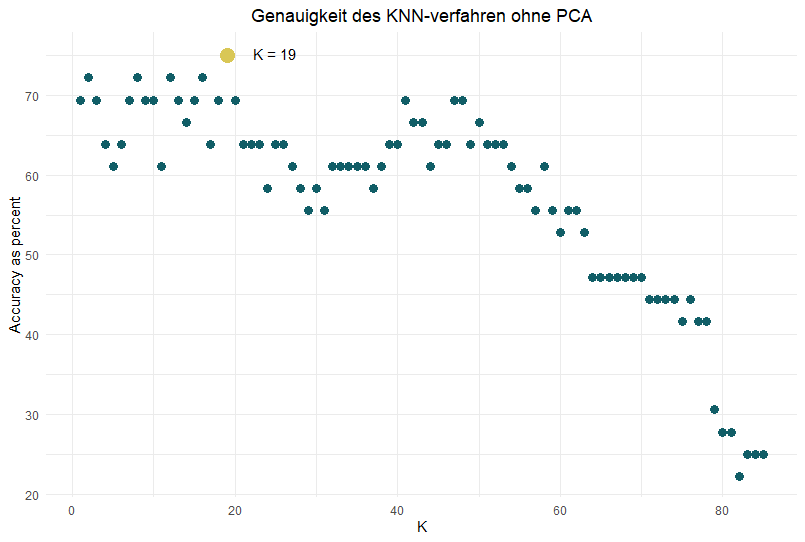
\includegraphics[width=\linewidth]{accuracy_knn_no_pca.png}
        \caption{Genauigkeit des Knn-Verfahren bei keiner Veränderung der Merkmale}\label{fig:acc_knn_normal}
    \end{subfigure}
    \vspace{1cm}
    \begin{subfigure}{\textwidth}
        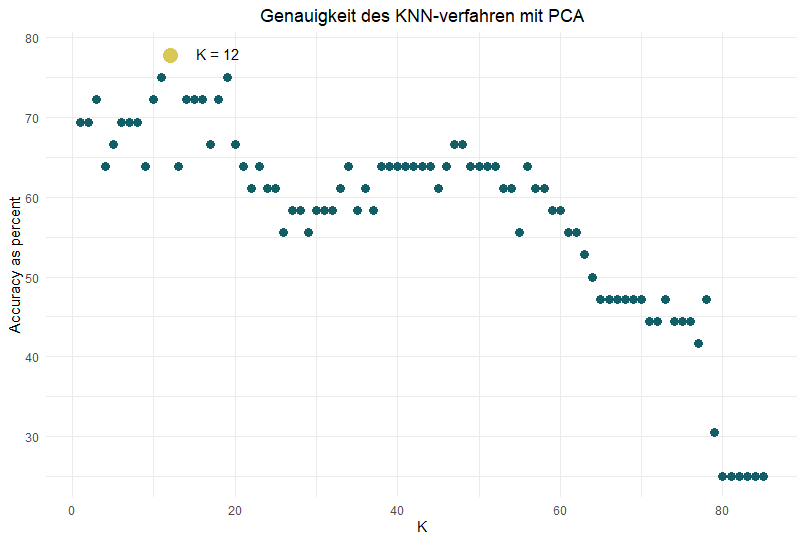
\includegraphics[width=\linewidth]{accuracy_knn_with_pca.png}
        \caption{Genauigkeit des Knn-Verfahren beim verwenden der ersten sechs Hauptkomponenten}\label{fig:acc_knn_pca}
    \end{subfigure}     
    \
\end{figure}

Damit scheint das Verfahren mit den Hauptkomponenten erstmal vorteilhaft.
Beim wiederholen der Ergebnisse fällt auf, dass die Genauigkeit der Verfahren schwankt. Grund dafür ist, dass das zur Erstellung des Knn-Modells verwendete Paket `Class' bei
einem Unentschieden in der Mehrheitswahl, die zugewiesene Klasse zufällig auswählt (\cite[p.4]{Ripley_2023}). Um herauszufinden, ob die Ergebnisse signifikant
unterschiedlich sind, verwende ich einen zwei Stichproben t-Test unter der Nullhypothese, dass die Verfahren sich in ihrer Genauigkeit im Mittelwert voneinander nicht unterscheiden. 
Das Ergebnis des Test ist ein $p$-Wert von $0,6975$, was bedeutet, dass die Differenz der Verfahren nicht groß genug ist, um
statistisch signifikant zu sein. Das Anwenden der Hauptkomponentenanalyse wäre somit nicht zwingend notwendig gewesen. 
Dies wird auch bei der Berechnung des AUC-Wertes klar. Dieser liegt bei dem Verfahren mit den originalen Merkmalen bei $0,8337$ und bei dem mit 
den Hauptkomponenten bei $0,773$.

\subsection{Spieler können im Team mehrere (oder keine) Rollen haben}
Fehler des Verfahrens und Ausreißer in den Daten können daher stammen, dass bestimmte Spieler nicht zwingend nur eine Rolle im Team übernehmen.
Ein gutes Beispiel dafür ist Finn `\textbf{karrigan}' Andersen, Ein sehr bekanntester Spieler in CS:GO.\@
Als Spieler ist karrigan sowohl \textbf{Entry} wie auch \textbf{IGL} für sein Team `Faze Clan' tätig (\cite{B_2023}). Im Bereich der Klassifikation macht diese Aufteilung der Rollen es somit schwer, eine eindeutige Zuweisung zu einer Rolle zu machen.
Herr Andersen ist jedoch keine Ausnahme, es gibt mehrere Spieler bei denen dies so ist. Es gibt zu dem auch Spieler die historisch keine feste Rolle in einem Team haben. Meine Quelle für die Rollen listet diese Spieler als `Rifler'.
Rifler sind wie erwähnt, Spieler die nicht strikt in die von mir definierten Rollen passen, sondern jemand, der die Rolle annimt, die das Team von ihm benötigt. Ich habe in meiner Verfahrensanwendung die Spieler ausgelassen, die die Rolle Rifler haben.
Für Spieler die zwei Rollen in einem Team haben, habe ich die Rolle verwendet für die sie in ihrem Team bekannt sind.

%------------------ Kapitel 4 -------------------------------------------------------------

\chapter{Fazit}
\section{Mögliche Anwendung der Ergebnisse}
\subsection{Empfehlungsdienst}
Valve bietet aktuell schon einen Dienst an, der einem Spieler einsicht über seine Performance gibt und diese in mehreren Statisitken zusammenfasst (\cite{Corporation_2021}).
Um die Features dieses Dienste zu erweitern kann basierend auf den Daten aus den Spielen der Knn-Algorithmus angewendet werden um eine Empfehlung für den Spieler
auszusprechen, welche Rollen am Besten zu dem Spieler passt. Innerhalb des Spieles ist es möglich mit anderen vorher unbekannten Spielern zusammenzuspielen, 
dieser Dienst nennt sich `Looking to play'. Das `Looking to play' könnte mit einer Rolleneinteilung erweitern werden um zu verhindern,
dass Spieler zusammen in Teams spielen, dessen Rollen sich überschneiden.
\section{Gelerntes}
Das Erlernte aus der Seminararbeit ist vielfältig. Ich habe gelernt, was für Datenquellen in einem weniger erforschtem Bereich existieren 
und wie ich diese Daten extrahieren kann um somit einen Datensatz zu erlangen der es ermöglicht Analysen durchzuführen. 
Mein Verständnis der angewandten Verfahren und deren Mathematischen Grundlagen wurde innerhalb der Recherche über die Verfahren erweitert. Das Verwenden von
\LaTeX{} zur Erstellung der Seminararbeit wird mich auf die Bachelorarbeit vorbereiten. Am Wichtigsten fand ich, dass das Erarbeiten der $R$ und $Python$ Skripte es mir ermöglicht 
explorative Datenanalyse innerhalb moderner und im Fach angewandten Programmiersprachen durchzuführen um somit mein Verständnis über die tatsächliche Anwendung der Verfahren
zu erweitern. Die Implikationen des Erzielten sind bedeutsam für meinen weiteren Werdegang als Studierender der Wirtschaftsinformatik/Wirtschaftwissenschaften.


%------------------ Literaturverzeichnis & Index -------------------------------

\backmatter{}
\printbibliography{}
\printindex												% Index (optional)
%------------------ Anhänge ----------------------------------------------------
\begin{appendix}

\printnoidxglossaries{}

\end{appendix}
\end{document}